\documentclass[11pt]{article}


%%%%%%%%%%%%%%%%5
\usepackage[utf8]{inputenc}
\usepackage{polski}
\usepackage{graphicx}
\usepackage{amsmath}
\usepackage{interval}
\usepackage[section]{placeins}
\usepackage{titlesec}
\titlelabel{\thetitle.\quad}


\topmargin=-0.45in
\evensidemargin=0in
\oddsidemargin=0in
\textwidth=6.5in
\textheight=9.0in
\headsep=0.25in

\linespread{1.1} % Line spacing


%%%%%%%%%%%%%%%%%

\date{Wrocław, \today}
\title{\LARGE\textbf{Pracownia P0}\\przykładowe sprawozdanie}
\author{Karolina Jeziorska}
        
\begin{document}
\maketitle

\newtheorem{tw}{Twierdzenie}


\thispagestyle{empty}     
\tableofcontents   

\vspace{1.5cm}\section{Przykładowy dział - tabela}
\subsection{Przykładowy poddział}
\subsection{Przykładowy poddział}

\begin{table}[!htb]
	\centering
	\begin{tabular}{|l|c|r|}\hline
	x & y & z \\ \hline
	4 & 557 & 6 \\ 
	4 & 557 & 6 \\ 
	45345 & 557 & 6 \\ 
	4 & 557 & 6 \\  
	45345 & 557 & 6 \\ 
	45345 & 557 & 6 \\ 
	4 & 557 & 6 \\  
	4 & 557435 & 6 \\ 
	7 & 8 & 95732 \\ \hline	
	\end{tabular}
	\caption{\label{tab:table-name}Tabela zawierająca liczby}
\end{table}


\section{Przykładowy dział - wykres}
\subsection{Przykładowy poddział}

Wykres funkcji \(y = x^2 - 4\) na przedziale \(\interval{-5}{5}\)

 
\begin{figure}[!htbp]
  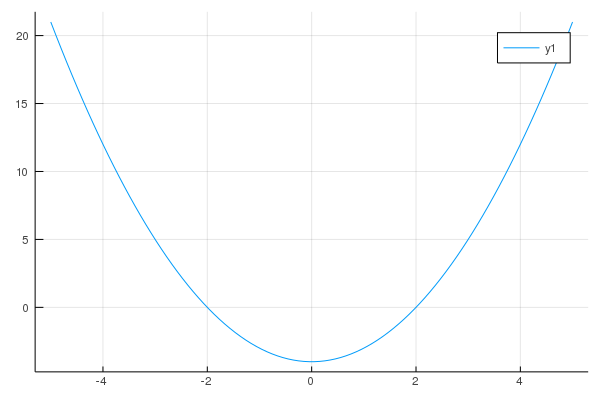
\includegraphics[width=15cm]{figura.png}
  \centering
  \caption{Wykres funkcji}
  \label{fig:wykres1}
\end{figure}



\section{Przykładowy dział - wzór}
Wzór Taylora:

\begin{multline}
f(x) = f(a) + \frac{x-a}{1!}f^{(1)}(a) + \frac{(x-a)^2}{2!}f^{(2)}(a) + \dots + \frac{(x-a)^n}{n!}f^{(n)}(a) + R_n(x,a) \\
= \sum_{k=0}^n(\frac{(x-a)^k}{k!}f^{(k)}(a)) + R_n(x,a)
\end{multline}



    
\end{document}


